% Gonski Lab -- SLAC Open House poster
% Built on the Gemini theme: https://rev.cs.uchicago.edu/k4rtik/gemini-uccs
% A fork of https://github.com/anishathalye/gemini

\documentclass[final]{beamer}

\pdfcompresslevel=0
\pdfobjcompresslevel=0

% ====================
% Packages
% ====================

\usepackage[T1]{fontenc}
\usepackage{lmodern}

\usepackage[scale=1.2, size=a0, orientation=portrait]{beamerposter}
\setlength{\paperheight}{46.8in}
\setlength{\paperwidth}{33.1in}

\usetheme{gemini}
\usecolortheme{stanford}
\usepackage{graphicx}
\usepackage{booktabs}
\usepackage{tikz}
\usepackage{pgfplots}
\pgfplotsset{compat=1.17}

\usepackage{siunitx}
\usepackage{enumitem}
\usepackage{multirow}
\usepackage{colortbl}
\usepackage{xcolor}
\usepackage{anyfontsize}
\usepackage[caption=false]{subfig}
\usepackage{amsmath}
\usepackage{makecell}

\usetikzlibrary{arrows.meta, positioning, shapes.geometric, calc}

% ====================
% Custom colors
% ====================
\definecolor{stageblue}{RGB}{41,98,163}
\definecolor{stagegreen}{RGB}{0,128,85}
\definecolor{stageorange}{RGB}{200,120,20}
\definecolor{stagepurple}{RGB}{100,60,150}
\definecolor{tcr}{RGB}{180,30,30}
\definecolor{tabheader}{RGB}{140,21,21}
\definecolor{tabheadertext}{RGB}{255,255,255}
\definecolor{tabrow1}{RGB}{255,245,245}
\definecolor{tabrow2}{RGB}{255,255,255}

\date{\today}

% Spacing
\setlength{\textfloatsep}{5pt}
\setlength{\abovecaptionskip}{2pt}
\setlength{\belowcaptionskip}{0pt}

% ====================
% Font overrides
% ====================
% Header type is scaled off the standard LaTeX sizes by \headfontscale percent,
% so the title and member lines can be nudged without jumping a whole size step
% (\LARGE -> \huge is far too big for the header box). anyfontsize, loaded above,
% permits the in-between sizes. Push this past ~115 and \headtextwidth needs
% widening too, or the student line will wrap.
\newcommand{\headfontscale}{110}
\makeatletter
\newcommand{\headscaled}[1]{%
  #1% select the base size, then rescale it
  \fontsize{\the\dimexpr\f@size pt*\headfontscale/100\relax}%
           {\the\dimexpr\f@baselineskip*\headfontscale/100\relax}%
  \selectfont}
\makeatother
\newcommand{\headtitlefont}{\headscaled{\LARGE}\bfseries}
\newcommand{\headauthorfont}{\headscaled{\normalsize}}

% % ====================
% Lengths
% ====================

\newlength{\sepwidth}
\newlength{\colwidth}
\setlength{\sepwidth}{0.025\paperwidth}
\setlength{\colwidth}{0.45\paperwidth}

\newcommand{\separatorcolumn}{\begin{column}{\sepwidth}\end{column}}

% ====================
% Helpers
% ====================

% Sub-heading inside a block. Both skips are starred: plain \vspace glue is
% discardable in vertical mode, so the trailing space vanished whenever a subhead
% was followed by \begin{columns} rather than by an ordinary paragraph.
\newcommand{\subhead}[1]{%
  \vspace*{0.7cm}%
  {\large\bfseries\color{cardinalred}#1}%
  \par\vspace*{0.65cm}}

% Shared height for the paired figures in the edge ML section
\newcommand{\edgefigheight}{7.8cm}

% Reserved space for a section that still needs content
\newcommand{\placeholder}[1]{%
  \vspace{0.3cm}
  \begin{center}
    \colorbox{boxgray}{%
      \parbox{0.92\columnwidth}{%
        \centering\vspace{1.2cm}%
        \textit{\textcolor{coolgray}{#1}}%
        \vspace{1.2cm}}}%
  \end{center}
  \vspace{0.3cm}}

% ====================
% Title
% ====================

\title{Machine Learning \& Microelectronics for\\New Physics Searches at Colliders}

% Two lines: seniors on the first, students on the second.
\author{%
  \textbf{PI:} Julia Gonski \quad \textbf{Postdocs:} Sagar Addepalli, Qibin Liu \\[0.8ex]
  \textbf{PhD:} Kenny Jia, Liangyu Wu \quad \textbf{Undergrads:} Gia Ancone, Deniz Yilmaz, Alexander Yue%
}

% No \institute and no \footercontent: the header carries the title and authors
% only, and the gemini footline template draws nothing when \footercontent is
% undefined, so the poster has no bottom band at all.

% ====================
% Headline layout
% ====================

% Override the gemini headline so the title/members block and both logos share one
% line: text flush left, then the SLAC wordmark, then the Stanford Block S. The
% flexible gaps are \hfil, so the three pieces spread evenly with no large void.
% These four knobs are all that need touching to rebalance the header. The SLAC
% wordmark is a 6:1 lockup, so matching the Block S height costs a lot of width:
% 28cm wide gives it ~4.7cm of height against the Block S at 6.4cm.
\newcommand{\headtextwidth}{0.53\paperwidth}   % width of the title/members block
\newcommand{\headslacwidth}{28cm}              % width of the SLAC wordmark
\newcommand{\headblockheight}{6.4cm}           % height of the Stanford Block S
\newcommand{\headlogogap}{2cm}                 % minimum gap between the two logos

\setbeamertemplate{headline}
{
  \begin{beamercolorbox}[wd=\paperwidth]{headline}
    \vskip6ex
    \hbox to \paperwidth{%
      \hskip\sepwidth
      \begin{minipage}[c]{\headtextwidth}
        \raggedright
        \usebeamerfont{headline}
        {\headtitlefont\usebeamercolor[fg]{headline title}\inserttitle\par}
        \vskip3ex
        {\headauthorfont\usebeamercolor[fg]{headline author}\insertauthor\par}
      \end{minipage}%
      \hfil
      \raisebox{-0.5\height}{%
        
\includegraphics[width=\headslacwidth]{stanford_logos/SLAC_primary_red.png}}%
      \hskip\headlogogap
      \hfil
      \raisebox{-0.5\height}{%
        
\includegraphics[height=\headblockheight]{stanford_logos/Block_S_2_color.png}}%
      \hskip\sepwidth
    }%
    \vskip6ex
    \ifbeamercolorempty[bg]{headline rule}{}{
      \begin{beamercolorbox}[wd=\paperwidth,colsep=0.5ex]{headline rule}\end{beamercolorbox}
    }
  \end{beamercolorbox}
}

% ====================
% Body
% ====================

\begin{document}

\begin{frame}[t]
\begin{columns}[t]
\separatorcolumn

\begin{column}{\colwidth}

  % ---------- 1. New physics searches ----------
  \begin{block}{Searching for New Physics}

    \begin{columns}[T]
    \begin{column}{0.7\columnwidth}
      We target \textbf{well-motivated BSM extensions undercovered at the LHC}:
      not unlikely, just hard to analyze. \textbf{Complex dark sectors} and
      \textbf{long-lived particles} are the prime examples.
    \end{column}
    \begin{column}{0.22\columnwidth}
      \centering
      
\includegraphics[width=0.75\columnwidth]{figures/openhouse/atlas_logo.png}
    \end{column}
    \end{columns}

    \subhead{Dark sector mediators}

    \begin{columns}[T]
    \begin{column}{0.53\columnwidth}
      \textbf{Dark matter} candidates can be produced in the decays of heavy scalar
      particles. Because they can be \textbf{long-lived}, they decay far from the
      primary proton collision point, leaving \textbf{displaced decay vertices}
      rather than tracks that all point back to one spot; new reconstruction
      techniques let us identify these vertices decaying to electron pairs in the
      ATLAS \textbf{inner tracker} and \textbf{calorimeter}.
    \end{column}
    \begin{column}{0.43\columnwidth}
      \centering
      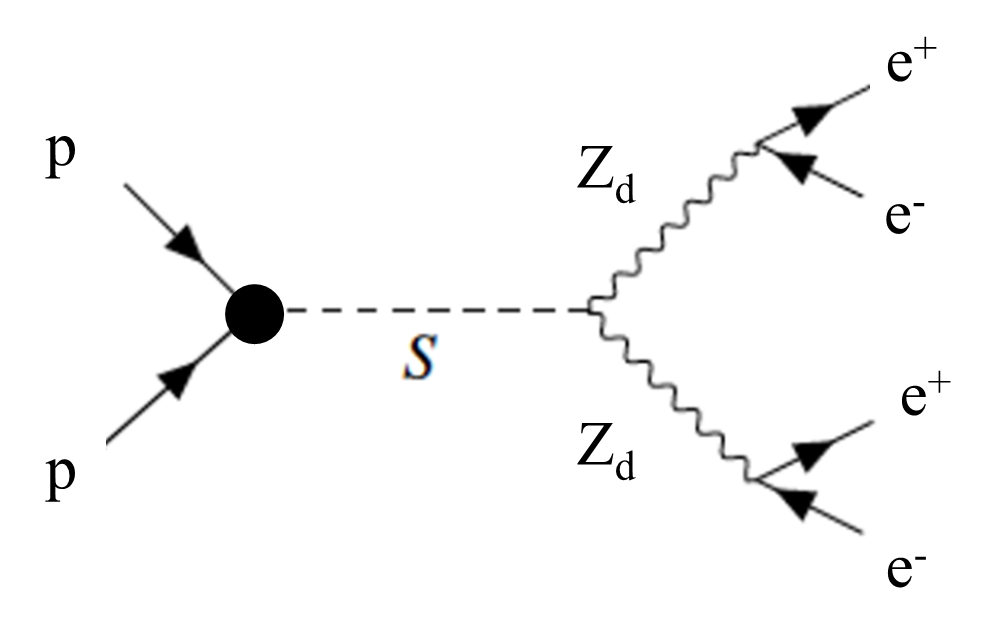
\includegraphics[width=0.88\columnwidth]{figures/openhouse/dark_sector_feynman.png}
    \end{column}
    \end{columns}

    \subhead{Anomaly detection in Higgs final states}

    The Higgs boson's \textbf{universal coupling to mass} makes it a broadly
    applicable portal to sectors beyond the Standard Model, and a natural anchor for
    anomaly detection. Our \textbf{HAXAD} (Higgs And X Anomaly Detection) strategy
    combines ML-based \textbf{feature embedding}, data-driven \textbf{background
    estimation} and \textbf{weakly supervised classification} to search for anomalies
    produced in association with a Higgs boson; a new inference framework now
    delivers \textbf{signal-agnostic} and signal-specific cross section limits that
    \textbf{match or exceed} the best limits of an equivalent cut-based search.

    \vspace{0.4cm}
    \begin{figure}
      \centering
      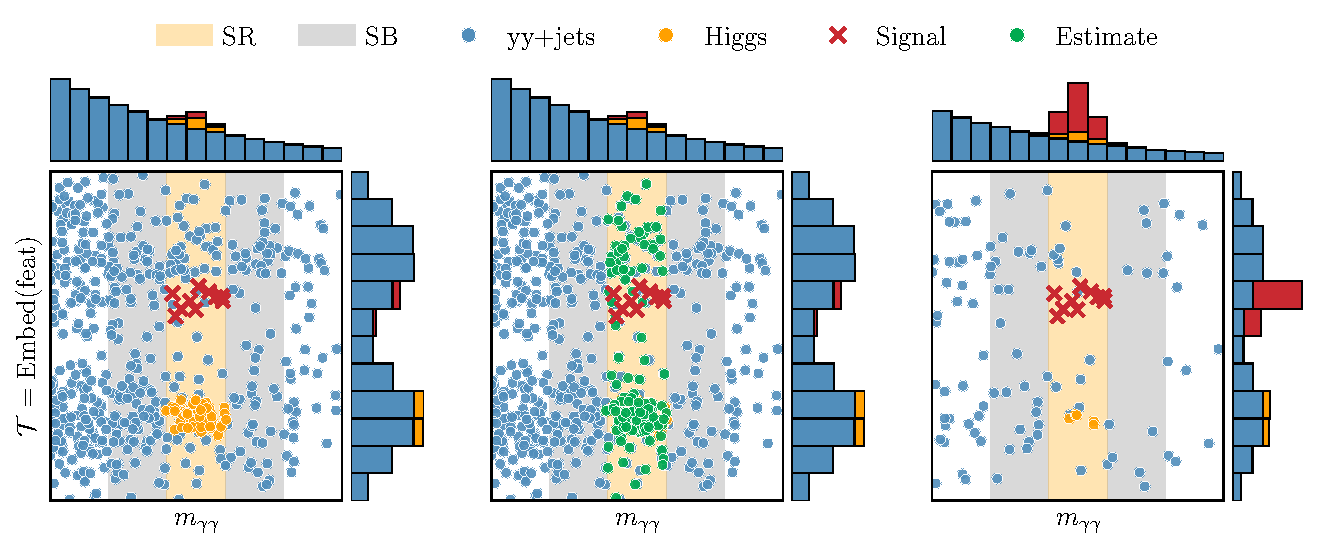
\includegraphics[width=0.80\columnwidth]{figures/openhouse/strategy.pdf}
    \end{figure}

  \end{block}


  % ---------- 2. Trigger anomaly detection ----------
  % Text/figure pairs rather than full-width stacked figures, to keep the section
  % compact without dropping any of the content.
  \begin{block}{Anomaly Detection in the ATLAS Trigger}

    The ATLAS \textbf{trigger} filters the LHC's \SI{40}{MHz} collision rate down to
    what can be stored to disk, making it the gatekeeper of all physics analyzed
    offline. Our group is \textbf{leading the effort} to bring real-time anomaly
    detection into that trigger: the first implementation entered data-taking in
    2025, collecting events \emph{orthogonal to existing trigger collection}, a phase
    space \textbf{never before seen} at the LHC.

    \vspace{0.4cm}
    Our \textbf{VAE-GAN} is trained on events described by the four-vectors of their
    constituent particles; the ones it reconstructs \emph{badly} are the ones worth
    saving.

    \vspace{0.4cm}
    \textbf{First ATLAS anomaly trigger has collected data, with Run 4 studies ongoing!}

    \vspace{0.4cm}
    \begin{figure}
      \centering
      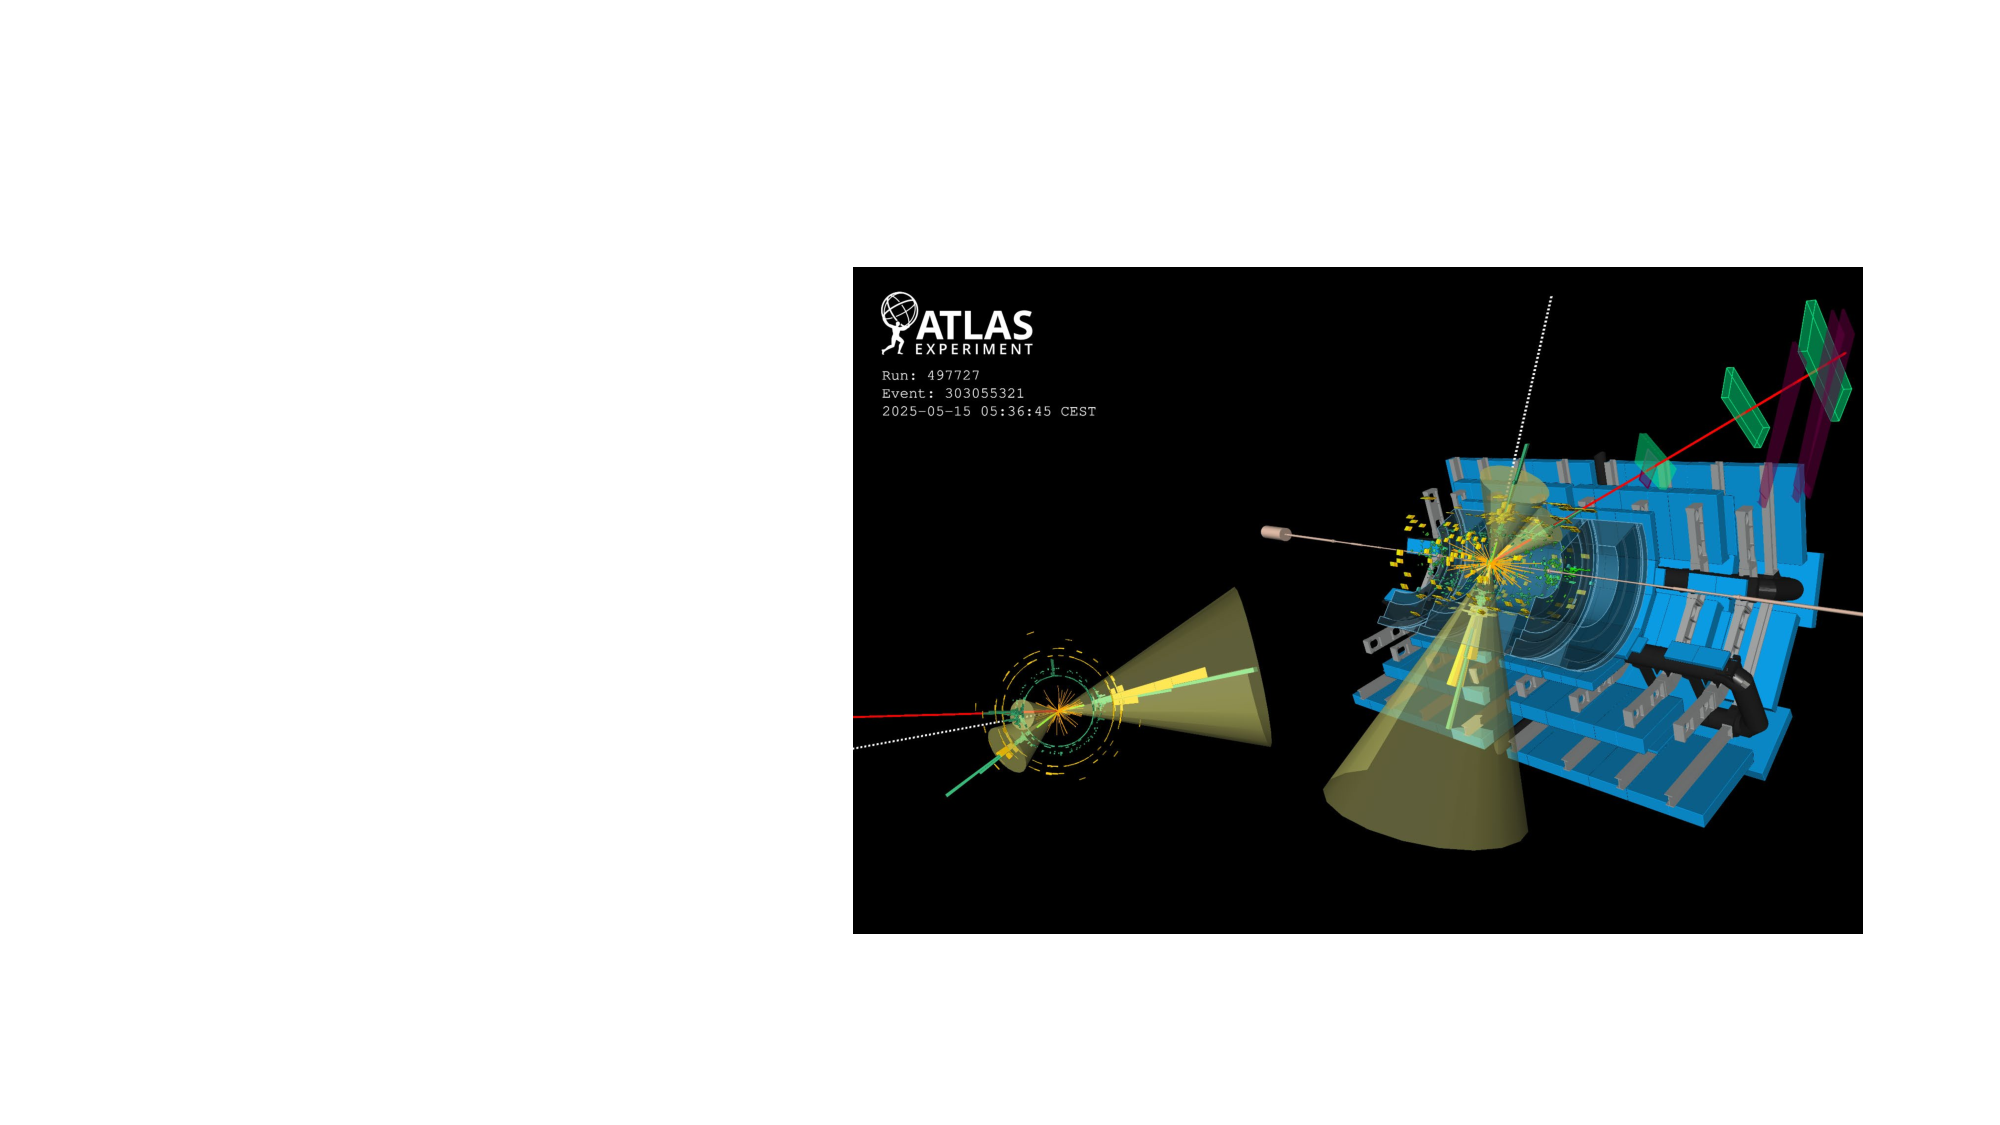
\includegraphics[width=0.6\columnwidth]{figures/openhouse/2025_eventDisplay.pdf}
    \end{figure}

  \end{block}


  % ---------- 3. Large-scale ML ----------
  \begin{block}{Foundation Models for Collider Physics}
    \vspace{1cm}
    % Opening sentence beside the logo, [c] so the two center against each other
    \begin{columns}[c]
    \begin{column}{0.62\columnwidth}
      We built \textbf{NEXUS}, a lightweight foundation model for collider data.
      With \textbf{no labels required}, it learns what an ordinary collision looks
      like from \textbf{20 million} LHC events, reading only the tracks that
      particles leave behind. That single backbone is then reused across many
      different analyses instead of training a new model from scratch every time,
      and it gets further on \textbf{far fewer labeled examples}.
    \end{column}
    \begin{column}{0.34\columnwidth}
      \centering
      
\includegraphics[width=\columnwidth]{figures/openhouse/NEXUS_logo.pdf}
    \end{column}
    \end{columns}

    \vspace{0.4cm}
    Most surprising of all, what it learns from particle collisions even transfers
    beyond physics: \textbf{gravitational waves}, \textbf{coastal flooding}, even
    \textbf{brain activity}. And at a fraction of the size of a transformer, it stays
    small enough to run in real time.

  \end{block}


\end{column}

\separatorcolumn

\begin{column}{\colwidth}

  % ---------- 4. Interpretable anomaly detection ----------
  \begin{block}{Interpretable Anomaly Detection}
    The \textbf{ORCA} framework is a \textbf{particle transformer} trained with
    \textbf{supervised contrastive learning}, which organizes events into an
    \textbf{embedding space} by Standard Model process; an \textbf{autoencoder} on
    that embedding then scores events that break the organization.

    \vspace{0.4cm}
    \begin{figure}
      \centering
      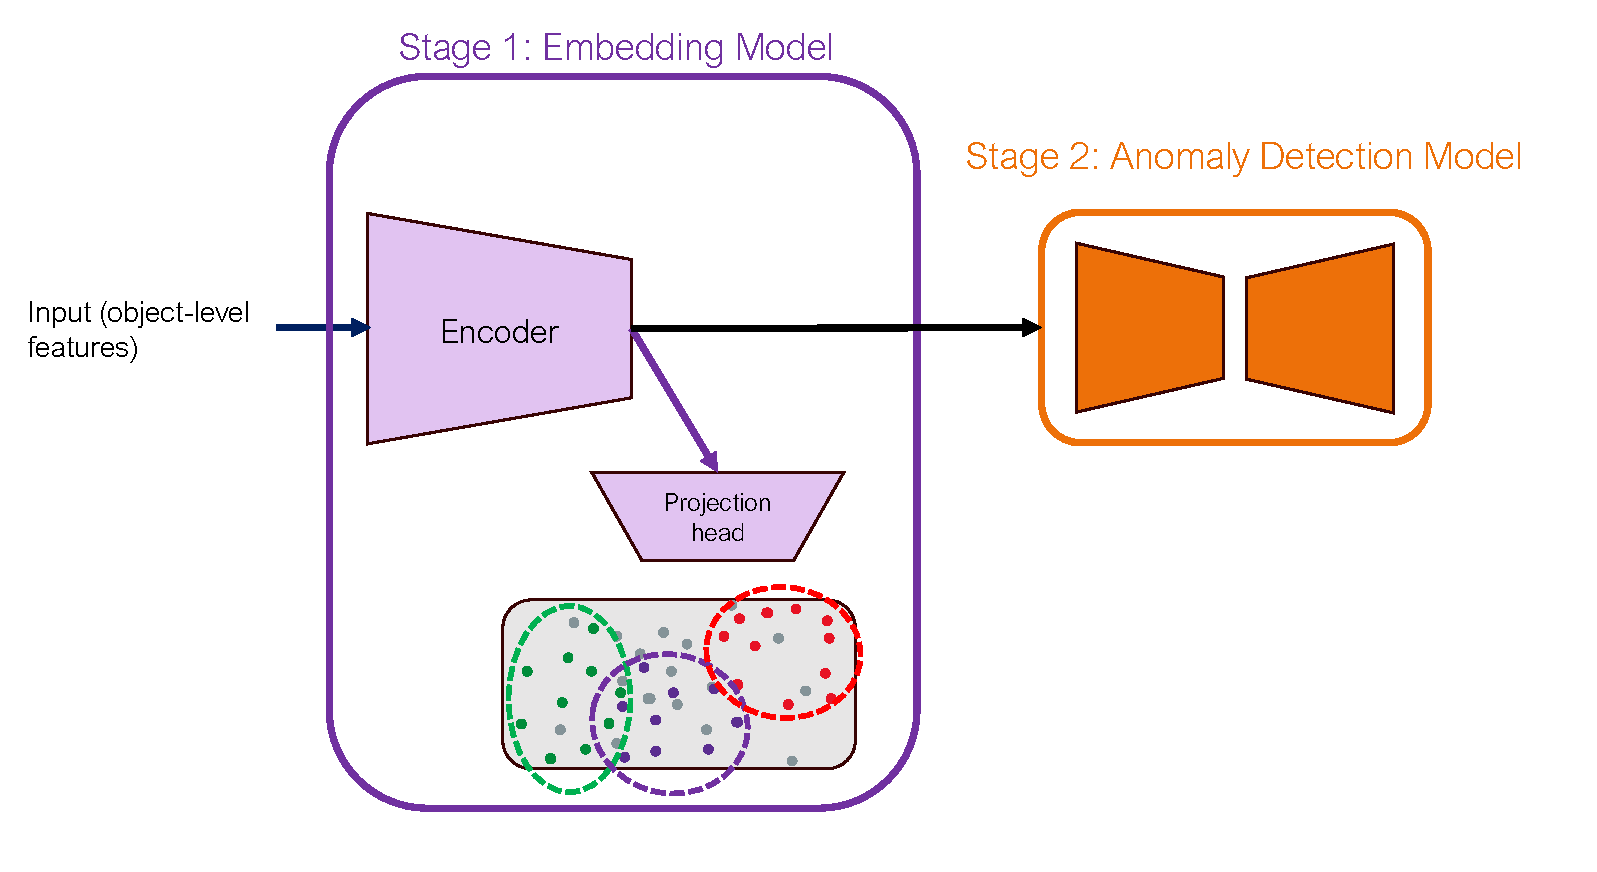
\includegraphics[width=0.75\columnwidth]{figures/openhouse/orca_two_stage_overview.pdf}
    \end{figure}

    A \textbf{template likelihood fit in the embedding space} measures the \textbf{composition} of the selected events in
    terms of known processes. 

  \end{block}


  % ---------- 5. Edge ML ----------
  \begin{block}{Edge ML \& Smart Detectors}

    At-source (\textbf{``edge''}) deployment of AI/ML can address the challenges of
    future ultra-high data rate experiments, but it demands novel solutions in
    microelectronics that deliver \textbf{reconfigurable digital logic} within
    stringent latency and power constraints.

    \vspace{0.4cm}
    \begin{figure}
      \centering
      % Fixed height on both so they line up; the pair is ~36cm of the 37.8cm column
      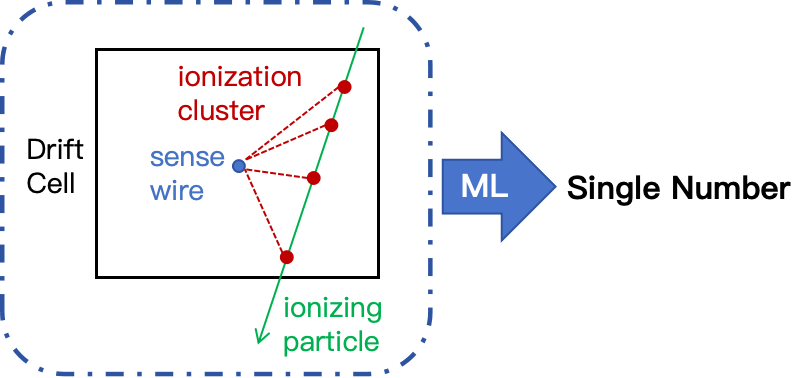
\includegraphics[height=\edgefigheight]{figures/openhouse/drift_cell_ml.png}%
      \hspace{1.5cm}%
      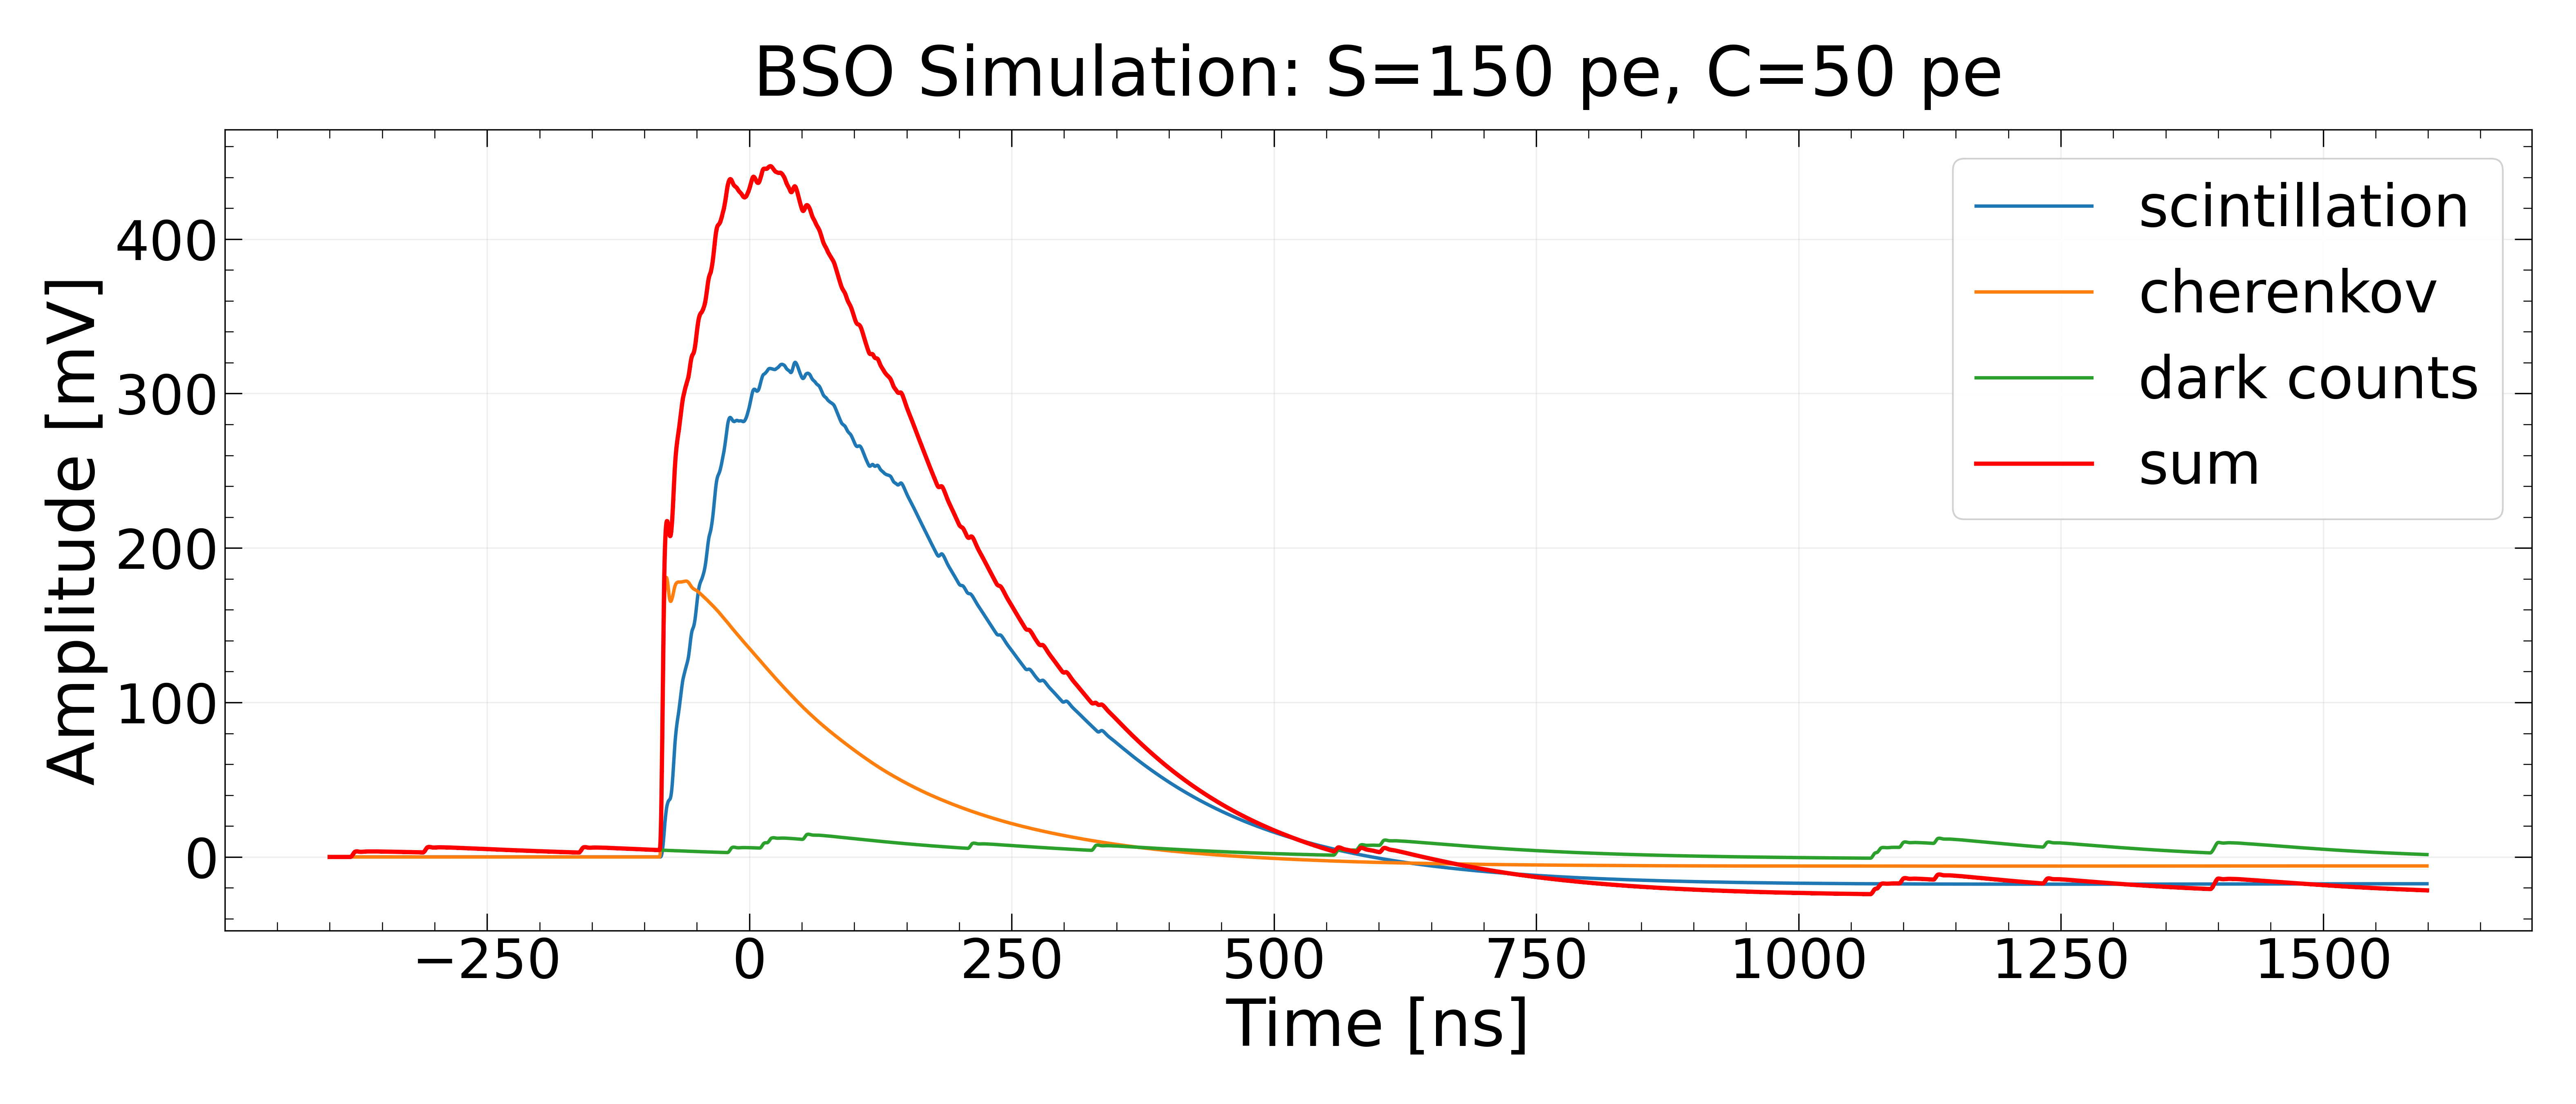
\includegraphics[height=\edgefigheight]{figures/wf_BSO.png}
    \end{figure}

    \vspace{0.4cm}
    \begin{columns}[T]
    \begin{column}{0.54\columnwidth}
      We are developing \textbf{embedded FPGA (eFPGA)} technology, which
      combines the benefits of an FPGA with the flexibility and processing power
      required for on-detector implementation.
    \end{column}
    \begin{column}{0.3\columnwidth}
      \centering
      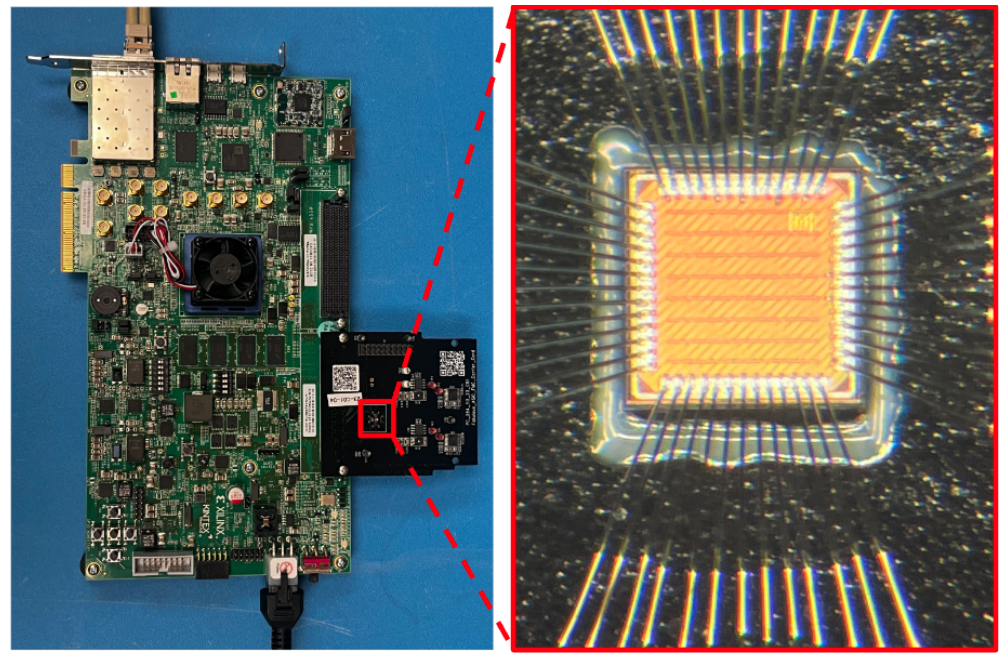
\includegraphics[width=\columnwidth]{figures/openhouse/efpga_board.png}
    \end{column}
    \end{columns}

    \vspace{0.4cm}
    In collaboration with engineers in SLAC's \textbf{Technology Innovation
    Directorate (TID)}, we explore eFPGA applications in advanced subsystems for
    future experiments such as \textbf{FCC-ee} --- including \textbf{drift chambers}
    and \textbf{dual-readout calorimeters} --- as well as beyond particle physics, in
    \textbf{photon science} and \textbf{quantum information science}.

    % \vspace{0.4cm}
    % Also with TID, we develop novel methods to implement machine learning on
    % \textbf{FPGAs}, targeting \textbf{ultra-fast inference} and \textbf{low power}
    % for applications like online data acquisition and processing.

    % \vspace{0.4cm}
    % \begin{figure}
    %   \centering
    %   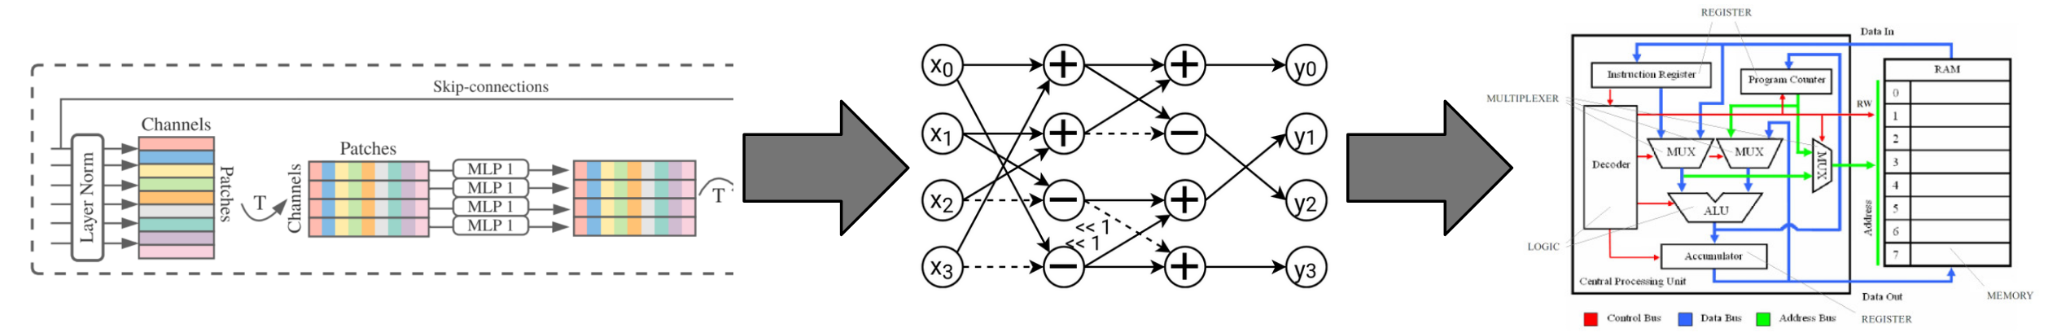
\includegraphics[width=\columnwidth]{figures/openhouse/mlpmixer_to_fpga.png}
    % \end{figure}

    \subhead{Distilling foundation models onto hardware}

    We train a \textbf{foundation model} on detector \textbf{waveforms}, then
    \textbf{compress and distill} it into a student network small enough to run on an
    FPGA at a fraction of the cost. Applying the same recipe to larger
    \textbf{HEP-ex} models is a route to \textbf{real-time foundation models},
    evaluated inside the latency budget of a trigger or a front-end ASIC.

  \end{block}


  % ---------- 6. Quantum ML ----------
  \begin{block}{Quantum Machine Learning}
    Quantum and quantum-inspired algorithms provide highly efficient frameworks for running real-time ML. We specialize in accelerating these algorithms on FPGAs, bringing the promise of \textbf{quantum advantage} to the hardware of today.
    \begin{figure}
      \centering
      % \hspace{1.5cm}%
      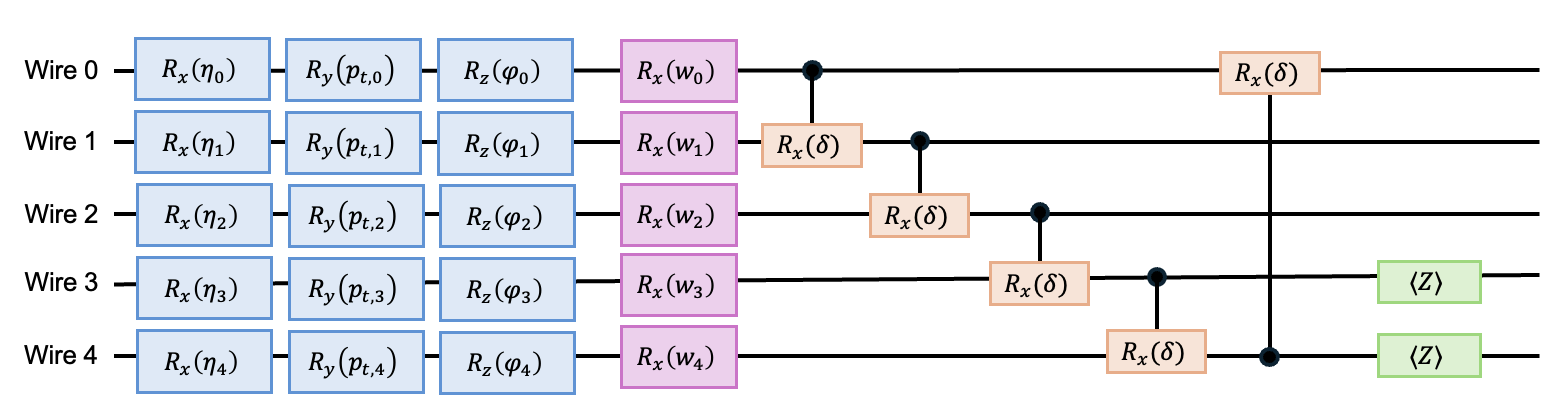
\includegraphics[height=\edgefigheight]{figures/openhouse/arch_qae_pqc.png}
    \end{figure}
    Quantum algorithms with just \textbf{tens of trainable parameters} can be accelerated on FPGAs within collider trigger constraints while outperforming neural networks on anomaly detection.

    While quantum computers mature, \textbf{quantum-inspired algorithms}, such as \textbf{tensor networks}, offer a classical pathway to exploit the entangled structure of collider data to enhance ML performance.
    \begin{figure}[!ht]
   \centering
   \begin{tikzpicture}[scale=2]
      %% Create a matrix site
      \tikzset
      {
      site/.style={circle, inner sep=0pt, outer sep=0pt, minimum width=1cm},
      selected site/.style = {site, fill=red!30},
      % nedge/.style = {-}
      }
      %% Sites
      \node[draw, site] (s0) at (0,0) {};
      \node[draw, site] (s1) at (1,0) {};
      \node[draw, site] (s2) at (2,0) {};
      \node[draw, site] (s3) at (3,0) {};
      \node[draw, site] (s4) at (4,0) {};
      \node[draw, site] (s5) at (5,0) {};
      \node[draw, site] (s6) at (6,0) {};
      \node[draw, site] (s7) at (7,0) {};
      \node[draw, site] (s8) at (8,0) {};
      \node[draw, selected site] (s9) at (9,0) {};
      \node[draw, site] (s10) at (10,0) {};
      \node[draw, site] (s11) at (11,0) {};
      \node[draw, site] (s12) at (12,0) {};
      \node[draw, site] (s13) at (13,0) {};
      \node[draw, site] (s14) at (14,0) {};
      \node[draw, site] (s15) at (15,0) {};
      \node[draw, site] (s16) at (16,0) {};
      \node[draw, site] (s17) at (17,0) {};
      \node[draw, site] (s18) at (18,0) {};
      %% Bonds
      \draw [thick] (s0) -- (s1) node[midway, above] {$b$} -- (s2) -- (s3) -- (s4) -- (s5) -- (s6) -- (s7) -- (s8) -- (s9) -- (s10) -- (s11) -- (s12) -- (s13) -- (s14) -- (s15) -- (s16) -- (s17) -- (s18)
      %% Incoming physical indices
      (s0) -- ++(0,1) node[midway, above=0.4cm] {$p_i$}
      (s1) -- ++(0,1)
      (s2) -- ++(0,1)
      (s3) -- ++(0,1)
      (s4) -- ++(0,1)
      (s5) -- ++(0,1)
      (s6) -- ++(0,1)
      (s7) -- ++(0,1)
      (s8) -- ++(0,1)
      (s9) -- ++(0,1)
      (s10) -- ++(0,1)
      (s11) -- ++(0,1)
      (s12) -- ++(0,1)
      (s13) -- ++(0,1)
      (s14) -- ++(0,1)
      (s15) -- ++(0,1)
      (s16) -- ++(0,1)
      (s17) -- ++(0,1)
      (s18) -- ++(0,1)
      %% Middle outline
      (s9) -- ++(0,-1) node[midway, below=0.4cm] {$p_o$};
   \end{tikzpicture}
\end{figure}
    \vspace{-1.5cm}
    Tensor networks can be run in tens of nanoseconds on FPGAs and exploit short- and long-range \textbf{entanglement structure of the underlying physics} to yield excellent signal to background separation. 
  \end{block}

\end{column}

\separatorcolumn

\end{columns}
\end{frame}

\end{document}
